\documentclass[a4paper,11pt]{article}
\usepackage{tabularx}
\usepackage{geometry}
\usepackage{xcolor}
\usepackage{physics}
\usepackage[most]{tcolorbox}
\usepackage{amsmath}
\usepackage{amssymb}
\usepackage{multicol}
\usepackage{float}
\usepackage{graphicx}
\usepackage{fancybox}
\usepackage{caption}
\usepackage{amsthm}
\usepackage{url}

\tcbuselibrary{breakable}
\geometry{left=1.4cm, top=0.8cm, right=1.2cm, bottom=1cm}

% Entorno para ejercicios con recuadro azul
\newtcolorbox{ejercicio}[1]{
    colback=white!8, colframe=blue!5!black,
    boxrule=0.75pt, arc=5pt, boxsep=10pt,
    title={\textbf{Ejercicio #1}}, fonttitle=\bfseries,
    breakable,
    before upper={\parindent15pt} % Añade sangría al texto
}

% Entorno para demostraciones con recuadro verde
\newtcolorbox{demostracion}[1]{
    colback=blue!5, colframe=gray!50!black,
    boxrule=0.75pt, arc=5pt, boxsep=10pt,
    title={\textbf{#1}}, fonttitle=\bfseries,
    breakable
}

\providecommand{\abs}[1]{\ensuremath{\left|#1\right|}}
\providecommand{\paren}[1]{\ensuremath{\left(#1\right)}}
\providecommand{\corche}[1]{\ensuremath{\left[#1\right]}}
\newcommand{\E}[1]{\mathbb{E}\left[#1\right]} % Esperanza
\newcommand{\LG}[1]{\mathcal{L}\left[#1\right]} % Transformada de Laplace
\newcommand{\LGV}[1]{\mathbb{L}\left[#1\right]} %
\newcommand{\V}[1]{\mathbb{V}\left[#1\right]} % Varianza
\newcommand{\COV}[2]{\mathbb{COV}\left[#1, #2\right]} % Covarianza
\NewDocumentCommand{\VA}{m}{\mathbf{#1}}

%----------HEADING-----------------
\begin{document}

\begin{tcolorbox}[colback=gray!10, colframe=black, boxrule=0.5pt, arc=5pt, boxsep=5pt]
\begin{tabularx}{\linewidth}{X r}
  \begin{tabular}[t]{@{}l@{}}
    \textbf{Introducción a la Ciencia de Datos} \\
    \textbf{Tarea I}
  \end{tabular}
  &\textbf{Antonio Barragán}\\
  &\textbf{Hazel Sánchez}\\
   & \textbf{Omar García Ramos} \\
\end{tabularx}
\end{tcolorbox}


%======================== DESCRIPCION DE LA BASE DE DATOS ====================

\section{Descripción de la base de datos}

\subsection*{Origen de los datos}

Estos datos forman parte del proyecto ISONET, que recopila isótopos estables de
carbono ($\delta^{13}C$) en celulosa de anillos de árboles de toda Europa. El
objetivo es estudiar el clima y la eficiencia en el uso del agua de los bosques
durante los últimos 400 años.

\subsection*{Estructura de los datos}

El conjunto de datos está organizado en un \texttt{DataFrame} con
\textbf{415 observaciones} (filas) y \textbf{26 variables} (columnas).
Contiene información sobre sitios de muestreo de árboles en Europa y sus
registros isotópicos ($\delta^{13}C$) a lo largo de varios años. Los valores
faltantes se indican como \texttt{NA}.

\begin{itemize}
    \item \textbf{Filas:} Cada fila representa un año, desde aproximadamente el
    año 1600 hasta 1995 (primeras 10 filas de metadatos).

    \item \textbf{Columnas:} Cada columna representa un sitio de muestreo en
    Europa.
\end{itemize}

\subsection*{Metadatos}

Sacamos los metadatos de cada variable de las primera 10 filas (incluyendo los
indices) del DataFrame y obtenemos la siguiente tabla (por practicidad ha sido
rotada y dividida).

\begin{table}[ht]
	\centering
	\caption{Metadatos - Información básica de los sitios}
	\label{tab:metadatos1}
	\begin{tabular}{|c|c|c|c|c|c|}
		\hline
		index & Site name & Country & Latitude & Longitude & Species \\
		\hline
		BRO & Bromarv & Finland & 60.00 & 23.08 & Quercus robur \\
		CAV & Cavergno & Switzerland & 46.35 & 8.6 & Quercus petraea \\
		CAZ & Cazorla & Spain & 37.93 & -2.97 & Pinus nigra \\
		COL & Col Du Zad & Morocco & 32.97 & -5.07 & Cedrus atlantica \\
		DRA & Dransfeld & Germany & 51.51 & 9.78 & Quercus petraea \\
		FON & Fontainebleau & France & 48.38 & 2.67 & Quercus petraea \\
		GUT & Gutuli & Norway & 62.00 & 12.18 & Pinus sylvestris \\
		ILO & Sivakkovaara & Finland & 62.98 & 31.27 & Pinus sylvestris \\
		INA & Inari & Finland & 68.93 & 28.31 & Pinus sylvestris \\
		%AHI & Perchtoldsdorf Wehrturm, Gaaden Glockenturm, Klosterneuburg
        %Glockenturm & Austria & 48.25 & 16.77 & Quercus petraea \\
		AHI & Perchtold... & Austria & 48.25 & 16.77 & Quercus petraea \\
		LAI & Lainzer Tiergarten & Austria & 48.18 & 16.20 & Quercus petraea \\
		LIL & Pinar de Lillo & Spain & 43.07 & -5.25 & Pinus sylvestris \\
		LOC & Lochwood & United Kingdom & 55.27 & -3.43 & Quercus petraea \\
		NIE1 & Niepolomice & Poland & 50.03 & 20.35 & Quercus robur \\
		NIE2 & Niepolomice & Poland & 50.03 & 20.35 & Pinus sylvestris \\
		PAN & Panemunes & Lithuania & 54.09 & 23.96 & Pinus sylvestris \\
		PED & Pedraforca & Spain & 42.23 & 1.70 & Pinus uncinata \\
		POE & Poellau & Austria & 47.31 & 15.81 & Pinus nigra \\
		REN & Renn & France & 48.02 & -1.83 & Quercus robur \\
		SER & Monte Pollino & Italy & 39.93 & 16.21 & Pinus leucodermis \\
		SUW & Suwalki & Poland & 53.95 & 23.25 & Pinus sylvestris \\
		VIG & Vigera & Switzerland & 46.05 & 8.77 & Pinus sylvestris \\
		VIN & Vinuesa & Spain & 42.00 & 2.75 & Pinus uncinata \\
		WIN & Windsor & United Kingdom & 51.43 & -0.61 & Pinus sylvestris \\
		WOB & Woburn & United Kingdom & 51.98 & -0.59 & Pinus sylvestris \\
		\hline
	\end{tabular}
\end{table}

\newpage

\begin{table}[ht]
	\centering
	\caption{Metadatos - Información temporal y de referencia}
	\label{tab:metadatos2}
	\begin{tabular}{|c|c|c|c|c|}
		\hline
		index & First year CE & Last year CE & elevation a.s.l. & Year CE \\
		\hline
		BRO & 1901 & 2002 & 5 & 13CVPDB \\
		CAV & 1637 & 2002 & 900 & 13CVPDB \\
		CAZ & 1600 & 2002 & 1820 & 13CVPDB \\
		COL & 1600 & 2000 & 2200 & 13CVPDB \\
		DRA & 1776 & 1999 & 320 & 13CVPDB \\
		FON & 1600 & 2000 & 100 & 13CVPDB \\
		GUT & 1600 & 2003 & 800 & 13CVPDB \\
		ILO & 1600 & 2002 & 200 & 13CVPDB \\
		INA & 1600 & 2002 & 150 & 13CVPDB \\
		AHI & 1600 & 1883 & n.s. & 13CVPDB \\
		LAI & 1812 & 2003 & 300 & 13CVPDB \\
		LIL & 1600 & 2002 & 1600 & 13CVPDB \\
		LOC & 1749 & 2003 & 175 & 13CVPDB \\
		NIE1 & 1627 & 2003 & 190 & 13CVPDB \\
		NIE2 & 1627 & 2003 & 190 & 13CVPDB \\
		PAN & 1816 & 2002 & 45 & 13CVPDB \\
		PED & 1600 & 2003 & 2120 & 13CVPDB \\
		POE & 1600 & 2002 & 500 & 13CVPDB \\
		REN & 1611 & 1998 & 100 & 13CVPDB \\
		SER & 1604 & 2003 & 1900 & 13CVPDB \\
		SUW & 1600 & 2004 & 160 & 13CVPDB \\
		VIG & 1675 & 2003 & 1400 & 13CVPDB \\
		VIN & 1850 & 1999 & 1950 & 13CVPDB \\
		WIN & 1763 & 2003 & 80 & 13CVPDB \\
		WOB & 1604 & 2003 & 10 & 13CVPDB \\
		\hline
	\end{tabular}
\end{table}


\subsection*{Estadísticas de los datos}

A continuación calculamos las estadísticas básicas sobre los datos y obtenemos.

\begin{table}[ht]
    \centering
    \caption{Estadísticas descriptivas de los datos}
    \label{tab:estadisticas_basicas}
    \begin{tabular}{|l|c|c|c|c|c|c|c|c|}
        \hline
        & count & mean & std & min & 25\% & 50\% & 75\% & max \\
        \hline
        %Year & 406.000 & 1802.500 & 117.346 & 1600.000 & 1701.250 & 1802.500 & 1903.750 & 2005.000 \\
        BRO & 102.000 & -25.505 & 0.671 & -27.200 & -26.000 & -25.500 & -25.000 & -23.800 \\
        CAV  & 365.000 & -24.122 & 0.489 & -25.500 & -24.400 & -24.200 & -23.800 & -22.500 \\
        CAZ  & 403.000 & -21.050 & 0.617 & -24.300 & -21.300 & -20.900 & -20.600 & -19.600 \\
        COL    & 280.000 & -20.756 & 0.435 & -25.300 & -21.000 & -20.800 & -20.500 & -19.600 \\
        DRA  & 226.000 & -23.788 & 0.856 & -26.000 & -24.300 & -23.800 & -23.300 & -21.000 \\
        FON  & 283.000 & -24.206 & 0.523 & -26.410 & -24.540 & -24.180 & -23.885 & -22.820 \\
        GUT  & 403.000 & -23.531 & 0.612 & -26.070 & -23.920 & -23.510 & -23.100 & -21.820 \\
        ILO & 403.000 & -23.603 & 0.689 & -26.000 & -23.900 & -23.500 & -23.100 & -22.300 \\
        INA  & 403.000 & -24.783 & 0.586 & -26.400 & -25.100 & -24.700 & -24.400 & -23.400 \\
        AHI & 284.000 & -24.694 & 0.828 & -27.600 & -25.100 & -24.600 & -24.200 & -22.700 \\
        LAI  & 192.000 & -25.060 & 0.786 & -27.700 & -25.525 & -25.100 & -24.600 & -23.000 \\
        LIL & 399.000 & -22.197 & 0.761 & -25.600 & -22.700 & -22.100 & -21.700 & -20.600 \\
        LOC  & 255.000 & -26.245 & 0.643 & -28.500 & -26.600 & -26.300 & -25.800 & -24.400 \\
        NIE1 & 377.000 & -25.256 & 1.145 & -28.710 & -25.920 & -25.160 & -24.520 & -20.460 \\
        NIE2 & 377.000 & -23.443 & 0.809 & -26.100 & -23.700 & -23.300 & -22.900 & -21.600 \\
        PAN  & 187.000 & -23.452 & 0.431 & -24.760 & -23.715 & -23.390 & -23.180 & -22.280 \\
        PED  & 401.000 & -22.006 & 0.622 & -24.170 & -22.350 & -22.000 & -21.580 & -20.340 \\
        POE  & 403.000 & -23.893 & 0.923 & -26.700 & -24.550 & -23.700 & -23.250 & -21.600 \\
        REN  & 367.000 & -24.435 & 0.870 & -26.680 & -25.115 & -24.280 & -23.720 & -22.640 \\
        SER & 400.000 & -22.210 & 0.697 & -24.300 & -22.500 & -22.100 & -21.700 & -20.700 \\
        SUW  & 405.000 & -23.080 & 0.811 & -25.100 & -23.700 & -23.100 & -22.500 & -20.900 \\
        VIG  & 328.000 & -23.281 & 0.597 & -25.100 & -23.700 & -23.300 & -22.800 & -21.800 \\
        VIN  & 150.000 & -22.573 & 0.832 & -25.000 & -22.900 & -22.400 & -22.000 & -21.100 \\
        WIN & 232.000 & -22.852 & 0.594 & -24.200 & -23.300 & -22.900 & -22.400 & -21.300 \\
        WOB  & 395.000 & -24.976 & 0.851 & -26.900 & -25.600 & -25.100 & -24.400 & -22.200 \\
        \hline
    \end{tabular}
\end{table}

\newpage

\subsection*{Valores Faltantes}

A continuación contamos el numero de valores faltantes y tenemos

\begin{table}[ht]
    \centering
    \caption{Tipos de datos, valores no nulos y faltantes por columna}
    \label{tab:info_datos}
    \begin{tabular}{|l|l|c|c|c|}
        \hline
        Columna & Tipo & No nulos & Valores faltantes & Porcentaje faltante \\
        \hline
        %Year & int64 & 406 & 0 & 0.000000 \\
        BRO & float64 & 102 & 304 & 74.876847 \\
        CAV  & float64 & 365 & 41 & 10.098522 \\
        CAZ  & float64 & 403 & 3 & 0.738916 \\
        COL    & float64 & 280 & 126 & 31.034483 \\
        DRA  & float64 & 226 & 180 & 44.334975 \\
        FON  & float64 & 283 & 123 & 30.295567 \\
        GUT  & float64 & 403 & 3 & 0.738916 \\
        ILO & float64 & 403 & 3 & 0.738916 \\
        INA  & float64 & 403 & 3 & 0.738916 \\
        AHI & float64 & 284 & 122 & 30.049261 \\
        LAI  & float64 & 192 & 214 & 52.709360 \\
        LIL & float64 & 399 & 7 & 1.724138 \\
        LOC  & float64 & 255 & 151 & 37.192118 \\
        NIE1 & float64 & 377 & 29 & 7.142857 \\
        NIE2 & float64 & 377 & 29 & 7.142857 \\
        PAN  & float64 & 187 & 219 & 53.940887 \\
        PED  & float64 & 401 & 5 & 1.231527 \\
        POE  & float64 & 403 & 3 & 0.738916 \\
        REN  & float64 & 367 & 39 & 9.605911 \\
        SER & float64 & 400 & 6 & 1.477833 \\
        SUW  & float64 & 405 & 1 & 0.246305 \\
        VIG  & float64 & 328 & 78 & 19.211823 \\
        VIN  & float64 & 150 & 256 & 63.054187 \\
        WIN & float64 & 232 & 174 & 42.857143 \\
        WOB  & float64 & 395 & 11 & 2.709360 \\
        \hline
    \end{tabular}
\end{table}

\newpage


Mostramos una grafica de como se distribuyen los datos faltantes en la tabla.
Cada casilla en blanco indica que es un valor faltante (NaN).

\begin{figure}[ht]
	\centering
	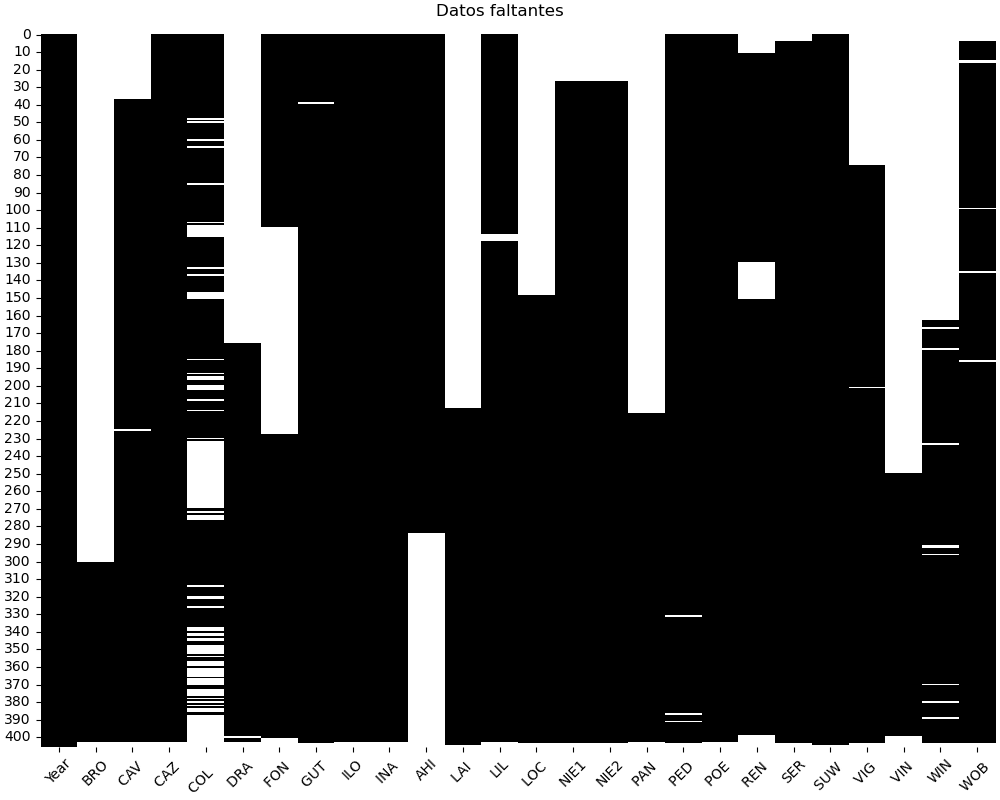
\includegraphics[width=0.7\linewidth]{figures/faltantes}
	\caption{Mapa de color - Datos faltantes}
	\label{fig:faltantes}
\end{figure}

\newpage

En la grafica podemos identificar patrones de que la medición de los datos en
ciertas variables falló de manera continua por ciertos periodos. Estos patrones
sugieren que algunas mediciones empezaron después de otras o terminaron antes
que otras. Además, en algunos casos las mediciones sólo tuvieron pausas.

Por otro lado, en otras variables los datos faltantes parecen seguir otra
distribución que sugieren fallas intermitentes en la medición de los datos, y
finalmente encontramos variables en las cuales no hay datos faltantes.

En nuestro caso, los \textit{NaN} pueden aparecer porque:
\begin{itemize}
    \item No se pudo tomar muestra ese año.

    \item El anillo no estaba presente o no era legible.

    \item No se llegó a ese año en la cronología de ese sitio.
\end{itemize}

Para el caso en que los datos faltantes sean por fallas intermitentes, el
análisis suguiere que el anillo no estaba presente o no era legible. Más
adelante consideraremos como manejar estos datos faltantes.

\newpage

\subsection*{Clasificación de las variables según su escala de medición}

A continuación se presenta la clasificación de cada variable de la base de datos
según su escala de medición. Se incluye una breve explicación del porqué de cada
clasificación.

\begin{table}[ht]
    \centering
    \caption{Clasificación de variables}
    \label{tab:clasificacion_variables}
    \begin{tabular}{|c|c|l|}
        \hline
        \textbf{Variable} & \textbf{Tipo} & \textbf{Justificación} \\
        \hline
        Site code & Nominal & Categorías sin orden (códigos de sitio) \\
        Site name & Nominal & Nombres sin orden jerárquico \\
        Country & Nominal & Países sin orden \\
        Latitude & Razón & Valor numérico con cero absoluto (grados) \\
        Longitude & Razón & Valor numérico con cero absoluto (grados) \\
        Species & Nominal & Nombre de especie sin orden \\
        Year CE & Intervalar & Años con intervalo constante, pero sin cero
        absoluto (no hay "año cero") \\
        $\delta^{13}$C & Razón & Valor numérico medido en $\%_o$\
        (per mil), con cero absoluto\\
        \hline
    \end{tabular}
\end{table}

Los datos de cada variable se miden en $\delta^{13}C$ que es la relación de
isótopos estables de carbono (13C/12C) en la celulosa del anillo de crecimiento.
Se expresa en $\%_o$ (per mil) respecto al estándar internacional VPDB.
\begin{itemize}
	\item Valores más negativos indican mayor fraccionamiento isotópico (ej: más
    humedad, menos estrés).

	\item Valores menos negativos indican menor fraccionamiento (ej: sequía,
    mayor eficiencia en el uso del agua).
\end{itemize}


\subsection*{Outliers}

Dada la naturaleza de nuestros datos, podemos considerar cada variable (medida
de $\delta^{13}C$ por localidad) como una serie de tiempo, para tener una mejor
interpretación de estas series graficamos el comportamiento de las estas series.

\begin{figure}[ht]
	\centering
	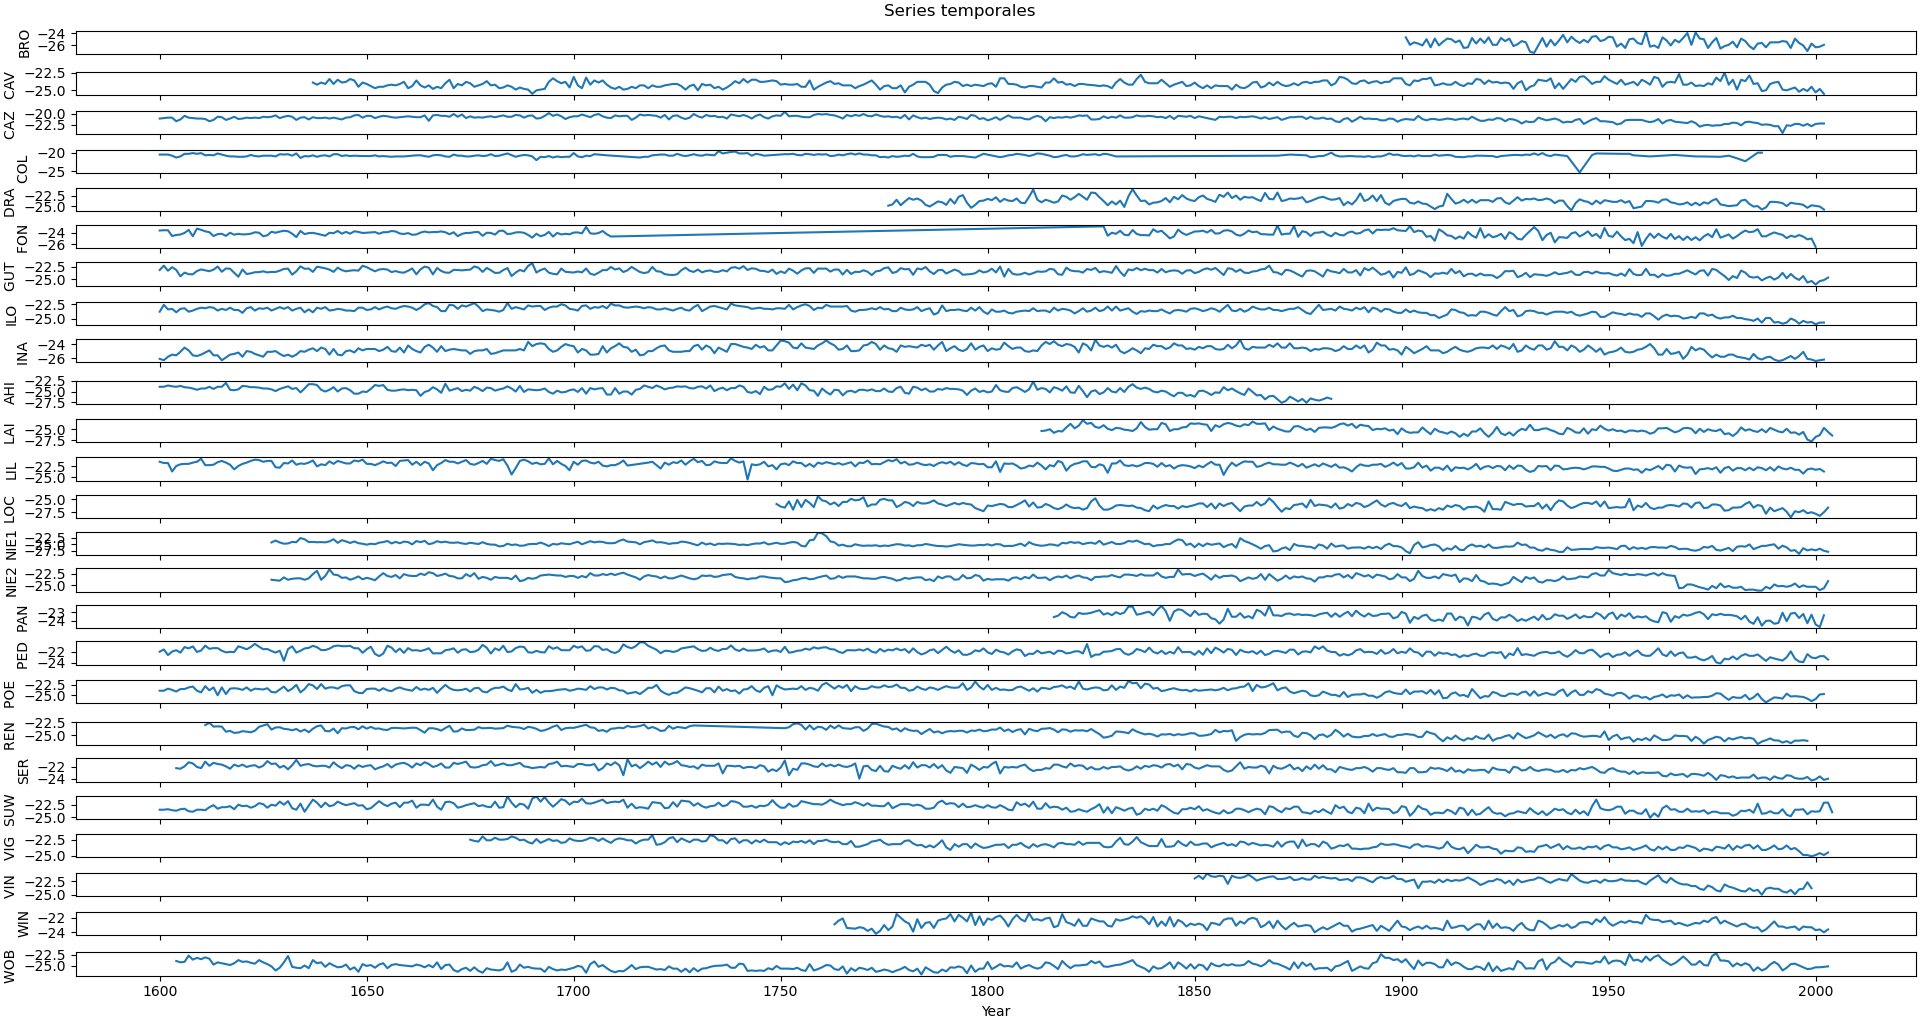
\includegraphics[width=0.95\linewidth]{figures/series.png}
	\caption{Grafica de cada serie}
	\label{}
\end{figure}

En las graficas de cada variable observamos algunos picos inusuales que pueden
sugerir la presencia de outliers, sin embargo estos picos ocurren en años
distintos para cada variable. Por lo cual, en caso de ser estos valores
outliers, no parecen tener que ver con algún factor físico en el entorno las
localidades donde se realizaron las mediciones.

Aún así, la observación anterior no es determinante ya que en nuestro caso
podemos notar que las variables no siguen un comportamiento suficientemente
similar entre ellas, esto lo vemos a través de la matriz de correlación,

\begin{figure}[ht]
	\centering
	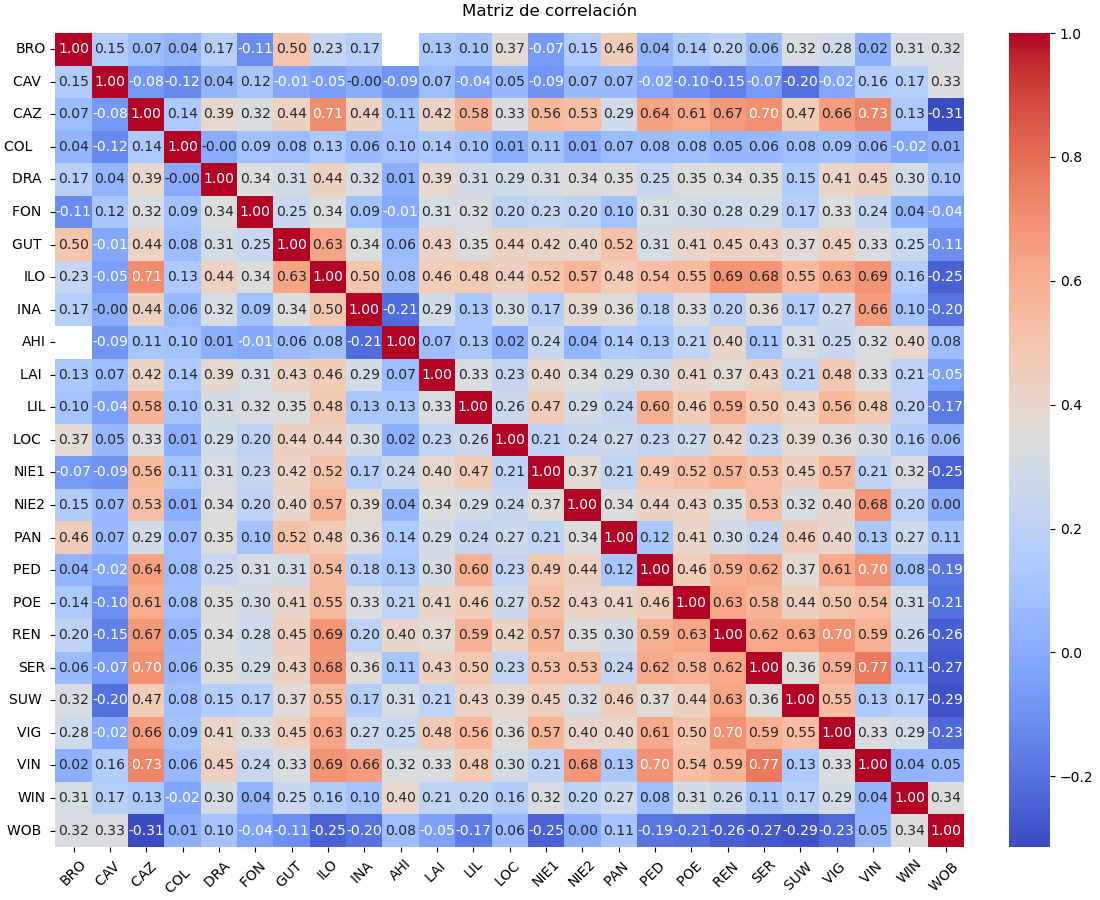
\includegraphics[width=0.7\linewidth]{figures/correlacion.png}
	\caption{Matriz de correlación}
	\label{}
\end{figure}

\newpage


Para buscar algún patrón que refleje ciclos podemos comparar las funciones de
auto-correlación de cada variable, sin embargo no lo realizaremos.


Por otro lado, para continuar con el análisis de outliers consideremos las
graficas de caja de cada variable.

\begin{figure}[ht]
	\centering
	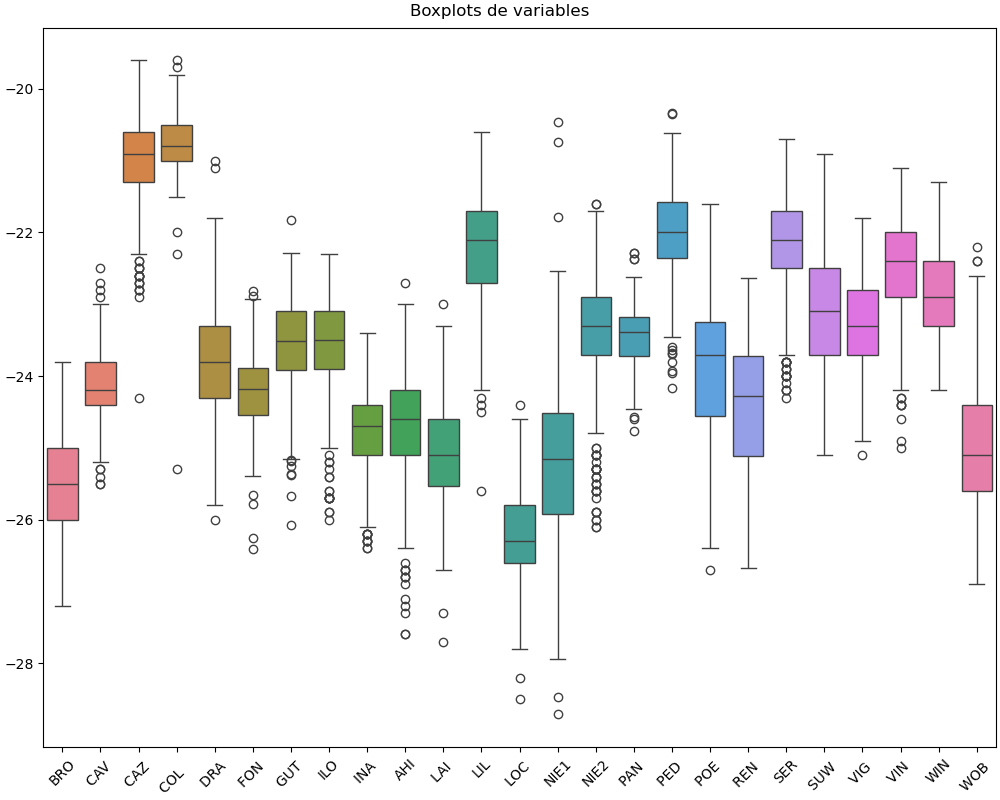
\includegraphics[width=0.7\linewidth]{figures/boxplots.png}
	\caption{Grafica de Boxplots}
	\label{}
\end{figure}

\newpage

En las graficas de caja notamos que en la mayoría de las localidades, las
mediciones parecen seguir una distribución simétrica (quizá una distribución
normal).

Además, notamos que en cada localidad, las mediciones tomadas y que son
candidatas a ser outliers se encuentran acumuladas por debajo de las otras
mediciones, esto sugiere fuertemente la existencia de algún otro fenómeno que
haga que las mediciones sean mas bajas en ciertos años.









\end{document}